\section{Введение}

Когда внешнее устройство генерирует сигнал, происходит исключительная ситуация
или исполняется специальная команда генерация программного прерывания процессор
должен прервать исполнение текущей задачи и вызвать обработчик прерывания
\footnote{Обатите внимание, мы пока не касаемся каким именно образом внешние
устройства посылают процессору сигнал, нас пока интересует только та часть общей
картины происходящего, за которую отвечает непосредственно процессор.}.

Для исключительных ситуаций используются первые 32 прерывания\footnote{Реально
используются только часть из них, неиспользуемые считаются зарезервированными.},
начиная с 32 прерывания до 256 не включительно, они доступны для произвольного
использования.

Код, на который процессор должен переключиться при получении прерывания,
называтеся обработчиком прерывания. В этом разделе мы каснемся того, как
сообщить процессору какой обработчик и когда вызывать, как должен выглядеть
обработчик прерывания, как запрещать/разрешать прерывания на процессоре.

\section{Таблица дескрипторов прерываний}

Таблица дескрипторов прерываний (так же известная как IDT) указывает процессору
какие обработчики прерываний за какие прерывания отвечают. Кроме того IDT
определяет, когда можно вызывать обработчик прерывания и в какой "режим" должен
перейти процессор перед тем как вызвать обработчик.

Указатель на IDT хранится в специальном регистре IDTR. Обращаться к этому
регистру с помощью обычных операций вроде mov нельзя, но для работы с ним
используются специальные инструкции lidt и sidt:

\begin{itemize}
  \item инструкция lidt записывает значение в IDTR;
  \item sidt считаывает значение из IDTR.
\end{itemize}

Значение в регистре IDTR имеет специальный вид:

\begin{lstlisting}
struct idt_ptr {
	uint16_t limit;
	uint64_t base;
} __attribute__((packed));
\end{lstlisting}

\begin{itemize}
  \item limit - размер таблицы в байтах минус 1;
  \item base - адрес таблицы\footnote{Я использую нотацию gcc, аттрибут packed,
значит, что компилятор не будет вставлять никаких padding-ов чтобы добиться
подходящего выравнивания для полей структуры.}.
\end{itemize}

Теперь касательно самой IDT. Таблица состоит из дескрипторов фиксированного
формата. На каждый из 256 возможных прерываний по одному дескриптору. Обратите
внимание, что размер таблицы максимум 256 записей, но никто не запрещает
использовать таблицу и меньшего размера. Главное следить за тем, чтобы не
произошло прерывание, для которого нет соответствующей записи в таблице.

Каждая запись в IDT состоит из 16 байт и имеет вид показанный на
Рис.~\ref{pic:idt}.

\begin{figure}
  \centering
  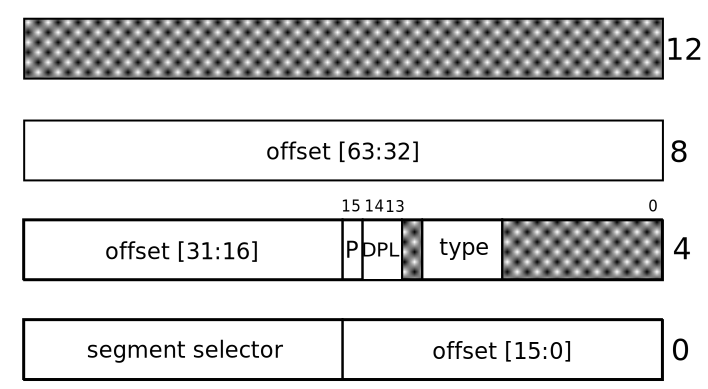
\includegraphics[width=0.8\textwidth]{idt.png}
  \caption{Запись в таблице IDT.}
  \label{fig:idt}
\end{figure}

\begin{itemize}
  \item offset - самое очевидное поле, оно указывает на адрес начала обработчика
  прерывания\footnote{Смотрите на этот адрес как на указатель на функцию
  обработчик.};
  \item segment selector - значение, которое будет загружено в сегментный
  регистр CS перед вызовом обработчика прерывания;
  \item P - бит присутствия, если он установлен, то запис воспринимается как
  валидная, в противном случае она невалидная и при получения прерывания для
  такой записи в IDT произойдет ошибка\footnote{Еще одно прерывание.};
  \item DPL (Descriptor Priviledge Level) - это поле используется для защиты
  обработчика прерывания от вызова в некоторых обстоятельствах;
  \item TYPE - дескрипторы бывают нескольких типов, нас, пожалуй, могут
  заинтересовать только два - Interrupt Gate (значение 14) и Trap Gate (значение
  15);
  \item IST - поле, которое отвечает за переключение стека при вызове
  прерываний, это полезная вещь с точки зрения безопасности, но нас она особо не
  будет интересовать, так что можно спокойно задавать это поле равным 0;
  \item все остальные поля зарезервированы и должны быть равны 0.
\end{itemize}

\subsection{Descriptor Priviledge Level}

Как вы возможно знаете, прерывания могут приходить не только от внешних
устройств, но также как реакция на какие-то ошибочные\footnote{Тут, забегая
далеко вперед, я должен сказать, что эти ситуация далеко не всегда являются
неожиданными ошибками, иногда ОС намернно ожидает исключения и они могут стать
частью логики работы ОС.} ситуация или генерироваться специальными инструкциями,
например, инструкцией int.

Инструкция int как аргумент принимает номер прерывания, обработчик которого
нужно вызвать. Это может создавать проблемы, например, представим, что
прерывание номер x настроено на работу с каким-нибудь внешним устройством,
например, сетевой картой. Пользовательское приложение может саботировать работу
системы намерено генерируя инструкцию int с аргументом x. Зачастую это
неприемлимо для ОС возволять какому-то приложению испортить жизнь всем
остальным приложениям. В конце концов, одна из задач ОС - изолировать приложения
друг от друга, чтобы ни одно из них не могло помешать другим\footnote{Стоит
отметить, что когда-то была довольно популярная ОС DOS, которая не изолировала
приложения друг от друга, так что все это довольно условно.}.

Так вот, поле DPL указывает уровень привелегий, которым должен обладать код
\footnote{Два младших бита регистра CS.}, чтобы он мог сгенерировать прерывание,
например, инструкцией int. Конечно, если прерывание сгенерировано устройством,
то эта проверка, конечно, не имеет смысла так как мы не можем делать никаких
предположений касательно кода исполняемого на процессоре в момент получения
сигнала от устройства, соответственно, и это поле будет проигнорировано в этом
случае.

Таким образом для всех аппаратных прерываний это поле должно иметь значение 0,
а, например, для прерыываний отведенных под системные вызовы это поле должно
иметь значение 3.

\subsection{Segment selector}

Назначение этого поля, на первый взгляд, очевидно - оно будет записано в регистр
CS. Но в чем назначение регистра CS? В 64-битном режиме x86 (он же Long Mode),
основное назначение - определять уровень привелегий\footnote{Что не значит, что
не нужно иметь соответсвующую запись в таблице GDT, даже если большая часть
полей }. Уровень привилегий кода определяется двумя младшими битами значения
регистра CS (0 - наибольший уровень привелегий, а 3 - наименьший).

Приключения начинаются, если уровень привилегий прерываемого кода, не совпадает
с уровнем привилегий обработчика прерываний, т. е. в ситуации если процессору
нужно сменить уровень привилегий, особенно, если мы переходим с более низкого
уровня привилегий к более высокому, например, от уровня 3 к уровню 0. И главная
проблема - это стек.

Стек является очень важным регионом памяти. На стеке зачастую храняться
локальные переменные вашего кода, на стек сохраняют адреса возврата, чтобы было
понятно куда возвращать управление после завершения функции. Другими словами,
стек во многом определяет работу вашего кода. Кроме всего прочего, в стек будет
сохранена информация о коде прерванном при вызове обработчика прерывания
\footnote{Интересный момент, в архитектуре ARM адрес возврата сохраняется не
в стек, а в специальны регистр, после чего его можно перенести куда угодно на
ваше усмотрение, впрочем, зачастую этот адрес всеравно попадет в стек, если
конечно вам вообще понадобится сохранить его куда-то еще.}.

А теперь представим ситуацию, когда обработчик прерывания прерывает
непривилгированный код, управление передается обработчику прерывания, т. е.
ядру ОС и ядро начинает сохранять на стек свою информацию. Но рано или поздно
обработчик прерывания завершится, и управление будет возвращено прерванному
коду, который в свою очередь может посмотреть, что же находится на стеке и,
таким образом, получить информацию из ядра ОС.

Таким образом, использовать стек пользовательского приложения для кода ядра ОС
идея не самая светлая\footnote{Впрочем, ядро ОС вполне может почистить стек за
собой.}, а процессор должен переключиться на использование новго стека
специально для ядра ОС. Поле IST как раз отвечает за это, но не только оно.
Однако на данной стадии нам не нужно об этом беспокоится по той простой причине,
что у нас, пока, есть только привелигированный код, а описанная выше проблема
нас не волнует.

\subsection{Маскировка прерываний и поле type}

Процессору можно сказать, чтобы он не принимал прерываний от внешних устройств.
Обратите внимание речь только о внешних устройствах, не отреагировать на
ошибочную ситуацию или на явный запрос от пользователя было бы очень странно.

Разрешено или нет процессору принимать прерывания определяется специальным битом
IF (номер 9 считая с 0) в флаговом регистре RFLAGS. Чтобы изменить значение
этого флага можно воспользоваться, например, инструкциями cli и sti.

Инструкция cli очищает этот флаг и запрещает процессору принимать прерывания,
а sti - обратная инструкция, которая устанавливает этот флаг и, соответсвенно,
разрешает прерывания\footnote{Не трудно запомнить, cli - clear interrupt flag,
а sti - set interrupt flag.}.

Как уже отмечалось, поле type нас в основном интересует для того чтобы выбрать
между Interrupt Gate и Trap Gate. В чем между ними разница? В случае Interrupt
Gate флаг IF будет очищен перед вызовом прерывания, т. е. прерывания от внешних
устройств будут запрещены. Trap Gate не запрещает прерывания, и, соответственно,
возможна ситуация когда один обработчик прерывания будет прерван другим
обработчиком прерывания, что само по себе не является проблемой.

\subsection{Обработчик прерывания}

Итак, offset указывает на начало обработчика прерывания, как должен выглядеть
этот обработчик прерывания. Перед тем как разбираться как должен выглядеть
обработчик прерывания, нам стоит понять в каком состоянии находится процессор,
когда обработчик получает управление.

Мы точно знаем, что в регистре CS содержится значение segment selector из
соответствующей записи в IDT, а в регистре RIP адрес обработчика прерывания,
записанный в поле offset записи IDT. Иногда мы так же можем знать один бит из
регистра RFLAGS, но это не так важно в данный момент.

Более существенно то, что находится на вершине стека. На
Рис.~\ref{fig:st_wo_err} и Рис.~\ref{fig:st_w_err} показаны два варианта
состояния стека. Для внешних устройств и программных прерываний возможен только
первый вариант\footnote{Инструкцией int мы можем сгенерировать прерывание с
любым номером, но стек всегда будет выглядеть одинаково.}, в то время как для
исключений возможны оба, какой именно используется определяется номером
исключения. Вариант показанный на Рис.~\ref{fig:st_w_err} используется для
исключений с номерами 8, 10-14 и 17.

\begin{figure}
  \centering
  \begin{subfigure}{0.4\textwidth}
    \includegraphics[width=0.9\textwidth]{st_wo_err.png}
    \caption{Stack without error code.}
    \label{fig:st_wo_err}
  \end{subfigure}
  \begin{subfigure}{0.4\textwidth}
    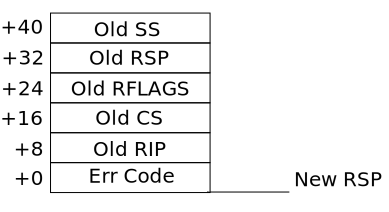
\includegraphics[width=0.9\textwidth]{st_w_err.png}
    \caption{Stack with error code.}
    \label{fig:st_w_err}
  \end{subfigure}
  \caption{Interrupt handler stack frame.}
  \label{fig:st_frame}
\end{figure}

Обратите внимание, что о состоянии преравнного кода нам изместно только значение
регистров CS, SS, RIP, RSP и RFLAGS. Где же хранится все остальное? На самом
деле нигде - все остальное вы должны сохранить самостоятельно. Другими словами
все остальные регистры, если вы собираетесь их менять в обработчике прерывания
вы должны самостоятельно сохранить, например, в стек. Восстановить сохраненную
информацию, опять же, ваша задача.

Другой важный момент - завершение обработчика прерывания. Обычно обработчик
прерывания завершается инструкцией iretq\footnote{На самом деле инструкция iret,
но у нее есть несколько вариаций, и iretq - та из них, которая нужна нам в
64-битном режиме работы.}. Инструкция iretq ожидает, что на врешине стека будет
находится информация показанная на Рис.~\ref{fig:st_wo_err}. Причем даже если
при вызове обработчика в стек был помещен код ошибки инструкция iretq ожидать
его не будет, и это ваша задача удалить его со стека.

Что делает инструкция iretq? Она берет информацию со стека и распихивает ее по
соответствующим регистрам - ничего особенного. Но из этого следует, в частности,
что вам не обязательно пользоваться инструкцией iretq, т. е. если вы сможете
повторить все тоже самое, что делает iretq без, собственно, iretq то это тоже
будет работать. И наоборот, нет никакого запрета на использование iretq за
пределами обработчика прерываний, если вам нужно то, что она делает.

Кроме того, для внешних прерываний, вам обычно нужно сообщить контроллеру
прерываний о том, что вы обработали прерывание, но эта часть истории будет
рассказана в другом разделе.

\subsection{Выводы}

Прочитав эту часть информации вы должны cуметь создать IDT, уметь запрещать и
разрешать прием прерываний и писать обработчики прерываний. Пока вы не знаете
как общаться с контроллером прерываний вы можете попрактиковаться на
исключениях. В частности, исключение деления на 0 очень легко сгенерировать
(делению на 0 соответсвует 0-ая запись в IDT\footnote{Полный список исключений
вы можете найти в документации Intel.}), а также вы можете воспользоваться
командой int.

Если вы будете практиковаться, пожалуйста обратите внимание какое значение RIP
попадает на стек в случае, если происходит деление на 0 и в случае использования
инструкции int.
